\documentclass[conference]{IEEEtran}
\IEEEoverridecommandlockouts
\usepackage{cite}
\usepackage{amsmath,amssymb,amsfonts}
\usepackage{tabularx}
\usepackage{algorithmic}
\usepackage{graphicx}
\usepackage{textcomp}
\usepackage{listings}
\usepackage{xcolor}
\usepackage{threeparttable}
\usepackage{array}
\usepackage{listings}
\usepackage{booktabs}
\usepackage{siunitx}
  \sisetup{
    table-format=1.3,
    round-mode = places,
    round-precision = 3,
  }
\usepackage{kantlipsum}
\def\BibTeX{{\rm B\kern-.05em{\sc i\kern-.025em b}\kern-.08em
    T\kern-.1667em\lower.7ex\hbox{E}\kern-.125emX}}
\begin{document}

\title{Project 1 - A Study on Privacy Preserving Libraries\\
}

\author{\IEEEauthorblockN{Ishaan Sathaye}
\IEEEauthorblockA{\textit{CSC 325 Intro to Privacy} \\
\textit{California Polytechnic State University, San Luis Obispo}\\
San Luis Obispo, U.S. \\
isathaye@calpoly.edu}
}

\maketitle

\begin{abstract}
This paper is a summary of 3 privacy-preserving technologies, which includes a
walk-through of OpenMinded's PySyft library as well as its implementation.
\end{abstract}

\section{Opacus, TensorFlow Privacy, and PySyft}

\subsection{Facebook's Opacus}

Developed by Facebook AI Research, Opacus is a open source library that is
designed to implement differential privacy easily into Py-Torch based machine
learning (ML) models. As there was a dire need for privacy preserving ML, this
framework enables the development on sensitive data without compromising the
privacy of individual data.

Applications of Opacus are abundant and span various industries with healthcare
and finance being its strong points. Regarding healthcare, this framework makes
sure that applications are compliant with privacy regulations, which enables
many of these developed platforms to achieve collaboration across institutions.
In the finance field, this library facilitates the development of the models on
financial data while at the same time ensuring the customers' their privacy. In
addition, this library has support for federated learning (FL), which makes it
even more valuable for research organizations nad educational institutions to
train models on diverse datasets. The main idea behind this library is that 
the data is protected by intervening on the parameters that are used by the 
model rather than handling the data \cite{b1}. As it offers a robust solution 
to the challenges of collaborative model training, Opacus is crucial for 
developing advanced ML applications in industries where privacy is key. 

\subsection{Google's TensorFlow Privacy}

Focusing on differential privacy with TensorFlow models, the TensorFlow Privacy
library is a versatile tool developed by Google to also address the preservation
of privacy in ML applications. The core behind this library is that Google
achieved privacy through this library by using differentially private
stochastic gradient descent. Similar to batch and normal SGD, this modification
of the algorithm prevents from exposing sensitive information such as
demographic information or other attributes \cite{b2}. 

As with Opacus, TensorFlow Privacy is also used in healthcare, finance, and 
also IoT applications. Similar to Opacus, this library offers compliance as well
as confidentiality when analyzing sensitive information in the finance and
healthcare industries. In addition, this library is also used in IoT
applications, since it enables the creation of systems that can learn from
sensitive data without compromising the privacy of the users. The unique
feature of TensorFlow Privacy is that it offers a variety of algorithms that
can be used to train models on sensitive data. In addition, this library also
offers a variety of tools that can be used to evaluate the privacy of the
models that are trained on sensitive data.

\subsection{OpenMinded's PySyft}

Developed by OpenMined, PySyft is a revolutionary framework that focuses on
addressing the challenges of secure and collaborative training across
decentralized datasets. As it is built on top of PyTorch, this library is
designed to be used with deep learning models. The main idea behind this
framework is that it enables the development of models on decentralized
datasets without the need for getting the user's data\cite{b3}, therefore keeping the
users' data on their devices.

As with the other two libraries, PySyft is also used in healthcare, finance,
and IoT applications. However, PySyft extends into other fields such as
e-commerce, telecommunications, and even government. Regarding e-commerce,
this library provides recommendations systems without compromising the privacy
of the users while at the same time ensuring a personalized experience. For
telecommunications, PySyft can analyze network data without centralizing
this very sensitive information, which in turn enhances the efficiency of
networks. In addition, PySyft can also be used in government applications to
predict analytics as well as do risk assessment. This open source library
showcases its versatility as it can be used in a variety of applications.

\subsection{Comparison}

\begin{table*}[h]
    \renewcommand{\arraystretch}{1.3}
    \caption{Comparison of Privacy-Preserving ML Libraries}
    \centering
    \begin{tabular}{|c|c|c|c|}
    \hline
    \textbf{Feature} & \textbf{Facebook Opacus} & \textbf{Google TensorFlow Privacy} & \textbf{OpenMinded PySyft} \\
    \hline
    \textbf{Purpose} & Privacy-preserving ML & Privacy-preserving ML & Privacy-preserving ML \\
    \hline
    \textbf{Framework Integration} & PyTorch & TensorFlow & PyTorch, TensorFlow \\
    \hline
    \textbf{Differential Privacy} & Yes & Yes & Yes \\
    \hline
    \textbf{Supported Algorithms} & DP-SGD & DP-SGD, PATE, Moments & DP-SGD, Federated Learning \\
    \hline
    \textbf{Communication Protocol} & N/A & gRPC, TFX & WebSockets, HTTP, gRPC \\
    \hline
    \textbf{Language Support} & Python & Python & Python, JavaScript \\
    \hline
    \textbf{Community Support} & Facebook & Google & OpenMinded \\
    \hline
    \textbf{Use Cases} & General-purpose & Various ML applications & Federated Learning, FLaaS \\
    \hline
    \textbf{License} & MIT & Apache 2.0 & Apache 2.0 \\
    \hline
    \textbf{Active Development} & Yes & Yes & Yes \\
    \hline
    \end{tabular}
\end{table*}

All 3 of these libraries support differential privacy to enhance privacy in ML
models. As well as that all 3 of these have a robust community support, which
makes it easier to develop applications on these libraries.

Regarding stark differences, Opacus is only compatible with PyTorch, while
TensorFlow Privacy is only compatible with TensorFlow. However, PySyft is
compatible with both PyTorch and TensorFlow, which makes it more versatile than
the other two libraries. A note to consider would be the use cases of each of
these libraries. Opacus is a general purpose library, while TensorFlow Privacy
is used in various ML applications. However, PySyft is used in federated
learning as well as FLaaS, which makes it more versatile than the other two
libraries.

\section{Walk-through of PySyft}

As PySyft is a very versatile library, which has capabilities such as FL,
additive secret sharing, and homomorphic encryption, this walk-through will
focus on the FL capabilities of this library.

\begin{figure}[h]
    \centering
    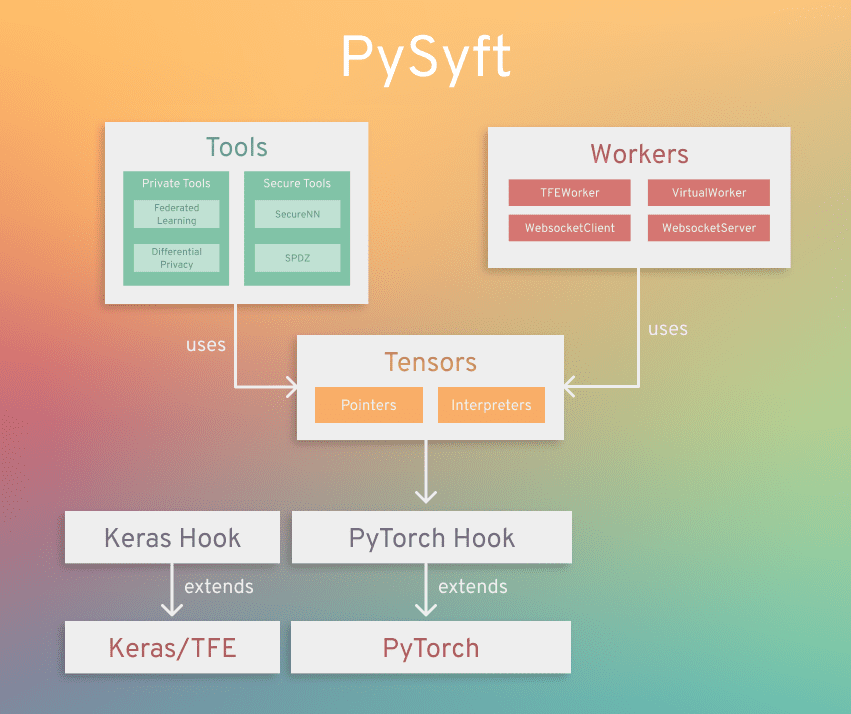
\includegraphics[width=0.8\linewidth]{overview.png}
    \caption{Overview of PySyft\cite{b4}}
    \label{fig:overview}
\end{figure}

\begin{figure}[h]
    \centering
    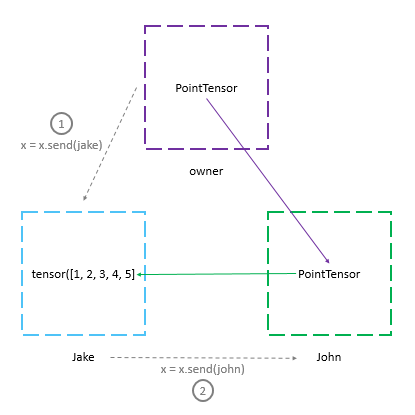
\includegraphics[width=0.8\linewidth]{send.png}
    \caption{Step 6: Sending the Model to the Workers\cite{b3}}
    \label{fig:send}
\end{figure}


\begin{enumerate}
    \item \textbf{Install PySyft:} Begin by installing the PySyft library on your system.
    \item \textbf{Create a Hook:} Establish a hook to extend PyTorch's functionality, acting as the link between PyTorch and PySyft.
    \item \textbf{Virtual Workers:} Define virtual workers representing different devices (local or remote) to hold data and models.
    \item \textbf{Load and Preprocess Data:} Divide and load the dataset onto different workers. Each worker holds a portion of the data.
    \item \textbf{Define a Model:} Specify your machine learning model using PyTorch.
    \item \textbf{Send Model to Workers:} Transmit the model to respective workers using PySyft's functionality.
    \item \textbf{Federated Training:} Train the model in a federated manner. Each worker performs training on its local data.
    \item \textbf{Aggregate Model Updates:} Combine model updates from different workers to form an updated global model.
    \item \textbf{Evaluate Federated Model:} Assess the performance of the federated model on a test set.
\end{enumerate}

In a nutshell, this walkthrough has 3 main steps to perform federated learning
using PySyft. First, you send the model to the device, then you train the model
\textbf{on the device} using the data that is \textbf{on the device}, and 
finally you get back the more intelligent model that is trained on the device.

\section{Implementation of PySyft}

For the implementation of PySyft, I used an example from the LearnOpenCV blog
by Jatin Prakash\cite{b4}. This example is federated learning in action on a
real like example such as the MNIST dataset. The MNIST dataset is a dataset of
handwritten digits, which is used to train models to recognize handwritten
digits. The scenario presented in this example is that there are 2 schools A and
B who do have have sufficient data to train a handwriting classifier on their
own. However, their combined data would be enough to train a model, given that
we train in a federated manner which will not expose the data to the other
school.

\subsection{Setup and Hooks}

Get the basic imports and import the PySyft library. Then, I need to create 2
schools A and B, which will be represented by 2 virtual workers. For the example
model, I will define a couple of arguments and a simple Convolution Neural 
Network (CNN).

\begin{lstlisting}[language=Python]
import torch
import torch.nn as nn
import torch.nn.functional as F
...
import logging

# Import PySyft and setup Workers
import syft as sy
hook = sy.TorchHook(torch)
school_A = sy.VirtualWorker(hook, id="A")
school_B = sy.VirtualWorker(hook, id="B")

# define some arguments and a simple CNN
args = {
    'use_cuda' : True,
    'batch_size' : 64,
    'test_batch_size' : 1000,
    'lr' : 0.01,
    'log_interval' : 10,
    'epochs' : 10
}

class Net(nn.Module):
def __init__(self):
    super(Net, self).__init__()
        
    self.conv = nn.Sequential(
        nn.ReLU(),
        nn.Conv2d(in_channels=32, ...),
        nn.ReLU()
    )
    self.fc = nn.Sequential(
        nn.Linear(in_features...),
        nn.ReLU(),
        nn.Linear(in_features...),
    )

    self.dropout = nn.Dropout2d(0.25)
    
def forward(self, x):
    x = self.conv(x)
    x = F.max_pool2d(x,2)
    x = x.view(-1, 64*12*12)
    x = self.fc(x)
    x = F.log_softmax(x, dim=1)
    return x
\end{lstlisting}

\subsection{Data Loading and Sending}

Since now the neural net is defined as well as the workers, I need to load and
send the data to workers. Transforming the data using \texttt{.federate()} will
make the data into a federated dataset, which will split the data set into 2 and
send this to the 2 schools. Then, I will define the train and test loaders for
the data. Some of the code is omitted for brevity.

\begin{lstlisting}[language=Python]
federated_train_loader = sy.FederatedDataLoader(
    datasets.MNIST('../data', train=True,
        transform=transforms.Compose([
            transforms.ToTensor(),
            ...
        ]))
    .federate((school_A, school_B)),
    batch_size=batch_size shuffle=True)
     
# this is the test loader
test_loader = torch.utils.data.DataLoader(
    datasets.MNIST('../data', ...([
            transforms.ToTensor(),
            ...
        ])),
batch_size=test_batch_size, shuffle=True)
\end{lstlisting}

\subsection{Training and Testing}

After, I defined the loaders which will be used to train and test the model, I
will define the training and testing functions. The training function will
iterate through the data and train the model on the data. The testing function
will test the model on the test data. Some of the code is omitted for brevity.

\begin{lstlisting}[language=Python]
def train(args, model, ...optimizer, epoch):
    model.train()

# iterate over federated data
for batch_idx, (data, target) in train_loader:

    # sending the model to the data location
    model = model.send(data.location)
    data, target = data.to(device), 
        target.to(device)
    optimizer.zero_grad()
    output = model(data)

    loss = F.nll_loss(output, target)
    loss.backward()

    optimizer.step()

    # get back the better updated model
    model.get()

    if batch_idx % 
        args['log_interval'] == 0:

        # compute the loss
        loss = loss.get()

        # print some metrics
        print(...)

def test(...):
    model.eval()
    test_loss = 0
    correct = 0
    with torch.no_grad():
        # compute the loss and accuracy

    test_loss /= len(test_loader.dataset)

    print(...)
\end{lstlisting}

\subsection{Training our Handwriting Classifier}

After defining the training and testing functions, I will define the model we
had defined earlier and the optimizer. Then, I will train the model for 10
epochs (as it was defined in the args) and test the model on the test data.

\begin{lstlisting}[language=Python]
# define the model and optimizer
model = Net().to(device)
optimizer = optim.SGD(model.parameters(), 
    lr=args['lr'])

# train/test the model to get some metrics
for epoch in range(1, args['epochs'] + 1):
        train(args, model, device,...epoch)
        test(model, device, test_loader)
\end{lstlisting}

After running the code, I get an output which tells me about the training and
testing of the model. In this output I can see the loss, accuracy, and other
metrics. In addition, I can see that the model was trained on the data that was
on the device, which is the main idea behind federated learning. However, the
main takeaway from this implementation is that the data was not exposed at
any point in the training process, which is the main idea behind federated
learning and using the PySyft library. The final output would be a model that
these schools can use to classify handwritten digits without exposing their
data to each other.


\section{Conclusion}

From this paper, I learned about 3 privacy-preserving libraries, which are
Opacus, TensorFlow Privacy, and PySyft. These libraries are used to develop
applications on sensitive data without compromising the privacy of the users.
In addition, I also learned about the implementation of PySyft, which is a
library that is used for federated learning. This library is used to train
models on decentralized datasets without exposing the data to the other
parties.

Some challenges that I faced during this project were the installation of the
libraries and also the implementation of PySyft. As I am currently taking
CSC 466: Knowledge Discovery from Data, I was able to understand the training
and testing of the model. However, I had to learn about the federated learning
coding paradigm, which was a challenge. Some future work that I would like to
do would be to implement the other features of PySyft such as additive secret
sharing and homomorphic encryption. In addition, I would like to implement the
other libraries such as Opacus and TensorFlow Privacy to get a better
understanding of these libraries.

\begin{thebibliography}{00}
    \bibitem{b1} VentureBeat, ``Facebook Open-Sources Opacus, a PyTorch Library 
    for Differential Privacy,'' August 31, 2020. \newline
    https://venturebeat.com/ai/facebook-open-sources-opacus-a-pytorch-library-for-differential-privacy/.
    \bibitem{b2} TensorFlow,``TensorFlow Privacy | Responsible AI Toolkit.'' n.d. Accessed November 15, 2023. \
    \newline https://tensorflow.google.cn/responsible\_ai/privacy/guide
    \bibitem{b3} OpenMined, ``Introduction to Federated Learning and Privacy Preservation Using PySyft and PyTorch,'' February 7, 2020. \newline
    https://blog.openmined.org/federated-learning-additive-secret-sharing-pysyft/.
    \bibitem{b4} LearnOpenCV, ``Federated Learning Using PyTorch and PySyft,'' May 25, 2020. \newline
    https://learnopencv.com/federated-learning-using-pytorch-and-pysyft/.
    \bibitem{b5} Github, ``Pytorch/Opacus,'' n.d. Accessed November 11, 2023. \newline
    https://github.com/pytorch/opacus.
    \bibitem{b6} Github, ``TensorFlow Privacy,'' n.d. Accessed November 11, 2023. \newline
    https://github.com/tensorflow/privacy
    \bibitem{b7} Github, ``OpenMined/PySyft,'' n.d. Accessed November 11, 2023. \newline
    https://github.com/OpenMined/PySyft.
\end{thebibliography}
    

\end{document}
